\newpage
\section{Виртуальные машины в эмулируемой сети}

GNS3 можно соединить с хостовой ОС Linux (на котором он запущен) и серверами в VirtualBox-е. Это значительно расширяет возможности по созданию сложных топологий с использованием роутеров Cisco, серверов с различными сервисами в VirtualBox и выходом в Интернет через хостовую ОС Linux. Виртуальные машины можно запускать и на QEMU, но VirtualBox предоставляет более удобный интерфейс для их создания и управления.

В данном примере используется сеть из трех соединенных между собой роутеров R1, R2 и R3, модели роутеров -- Cisco 2651XM. R1 через облако C1 подсоединен к родному хосту Ubuntu (на котором запущен GNS3). Для этой машины имя будет ubox. Через этот хост проводится синхронизация времени по ntp, закачка на роутеры дополнительных файлов по tftp и доступ в Интернет. Через облако С2 сеть подключена к виртуальной машине в VirtualBox. В данном случае это Debian с установленным FreeRADIUS для аутентификации и авторизации на роутерах и Syslog сервером для логов. Топология сети приведена на рисунке 8.

\begin{figure}[h!]
\centering
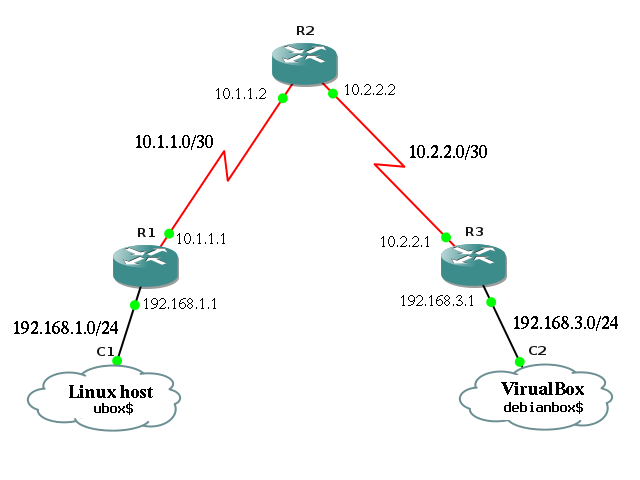
\includegraphics[scale=1]{res/pic008}
\caption{Топология сети}
\end{figure}

Для реализации этой схемы, произведём установку утилиты tunctl для создания и управления TUN/TAP виртуальными сетевыми интерфейсами:

\begin{Verbatim}[frame=single]
ubox$ sudo apt-get install -y uml-utilities
\end{Verbatim}

И утилиту brctl для создания и настройки сетевых мостов:
\begin{Verbatim}[frame=single]
ubox$ sudo apt-get install -y bridge-utils
\end{Verbatim}

Теперь создаем и конфигурируем виртуальные сетевые интерфейсы:
\begin{itemize}
\item tap0 -- для связи с Linux-ом, на котором и запущен GNS3.
\item tap1 -- для связи через мост с гостевыми машинами VirtualBox-а.
\end{itemize}
\begin{Verbatim}[frame=single]
ubox$ sudo tunctl -t tap0 -u username
ubox$ sudo tunctl -t tap1 -u username
ubox$ sudo ip addr add 192.168.1.1/24 dev tap0
ubox$ sudo ip link set up dev tap0
\end{Verbatim}

Обеспечим привязку интерфейсов к облаку (рис. 9)

\begin{figure}[h!]
\centering
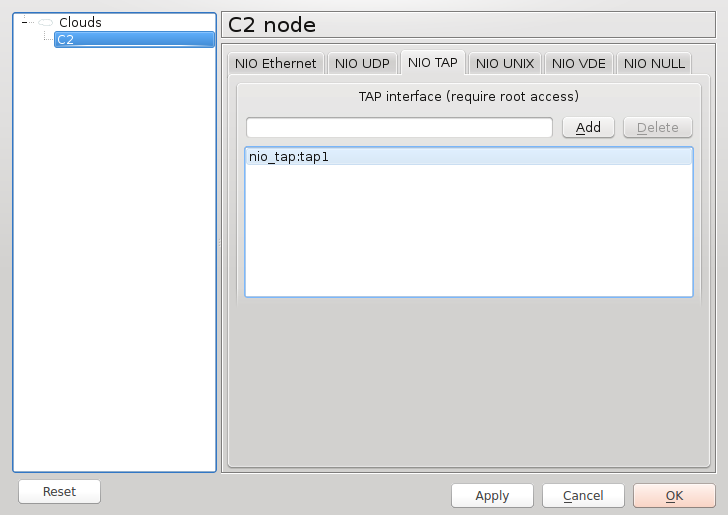
\includegraphics[scale=0.85]{res/pic009}
\caption{Привязка виртуальных интерфейсов}
\end{figure}

Связь с VirtualBox-ом осуществляется через мост br0, который состоит из виртуального Host-only интерфейса vboxnet0 и уже созданного tap1.
\begin{Verbatim}[frame=single]
ubox$ sudo brctl addbr br0
ubox$ sudo brctl addif br0 tap1
ubox$ sudo brctl addif br0 vboxnet0
ubox$ sudo ifconfig br0 192.168.3.4 netmask 255.255.255.0 up
\end{Verbatim}

Для связи всего этого хозяйства c хостовым Linux-ом на нем необходимо прописать маршрутизацию в используемые подсети:
\begin{Verbatim}[frame=single]
ubox$ sudo route add -net 10.1.1.0/24 gw 192.168.1.1
ubox$ sudo route add -net 10.2.2.0/24 gw 192.168.1.1
ubox$ sudo route add -net 192.168.3.0/24 gw 192.168.1.1
\end{Verbatim}

Теперь перейдём к настройке роутеров. На всех роутерах нужно прописать роутинг на подсети (или использовать протоколы динамической маршрутизации). Мы используем проприетарный цисковский протокол динамической маршрутизации EIGRP. Настройка выглядит следующим образом:

Для R1 --

\begin{Verbatim}[frame=single]
R1# conf t
R1(config)# router eigrp 1
R1(config-router)# passive-interface FastEthernet0/0
R1(config-router)# network 10.1.1.0 0.0.0.3
R1(config-router)# network 192.168.1.0
R1(config-router)# no auto-summary
R1(config-router)# exit
R1(config)# ip route 0.0.0.0 0.0.0.0 FastEthernet0/0
\end{Verbatim}

Для R2 --

\begin{Verbatim}[frame=single]
R2# conf t
R2(config)# router eigrp 1
R2(config-router)# network 10.1.1.0 0.0.0.3
R2(config-router)# network 10.2.2.0 0.0.0.3
R2(config-router)# no auto-summary
R2(config-router)# exit
R2(config)# ip route 0.0.0.0 0.0.0.0 Serial0/0
\end{Verbatim}

Для R3 --

\begin{Verbatim}[frame=single]
R3# conf t
R3(config)# router eigrp 1
R3(config-router)# passive-interface FastEthernet0/0
R3(config-router)# network 10.2.2.0 0.0.0.3
R3(config-router)# network 192.168.3.0
R3(config-router)# no auto-summary
R3(config-router)# exit
R3(config)# ip route 0.0.0.0 0.0.0.0 Serial0/0
\end{Verbatim}

На Debian-е (запущенном в VirtualBox) устанавливается сетевой адрес и шлюз по умолчанию:
\begin{Verbatim}[frame=single]
debianbox$ ifconfig eth0 192.168.3.3 netmask 255.255.255.0 up
debianbox$ route add default gw 192.168.3.1
\end{Verbatim}

Для того, чтобы работал Интернет через хостовый Linux нужно применить следующие правила (eth0 — внешний интерфейс).
\begin{Verbatim}[frame=single]
echo 1 > /proc/sys/net/ipv4/ip_forward
ubox$ sudo /sbin/iptables -t nat -A POSTROUTING -o eth0 -j MASQUERADE
ubox$ sudo /sbin/iptables -t nat -A POSTROUTING -o eth0 -j LOG
ubox$ sudo /sbin/iptables -A FORWARD -i eth0 -o tap0 -m state --state 
                                             RELATED,ESTABLISHED -j ACCEPT
ubox$ sudo /sbin/iptables -A FORWARD -i tap0 -o eth0 -j ACCEPT
\end{Verbatim}

На базе данного примера можно строить сетевые топологии еще больше и сложнее. GNS3 позволяет эмулировать ASA, PIX, IPS, JunOS; простые Ethernet, ATM и Frame Relay коммутаторы; позволяет перехватывать пакеты с помощью Wireshark.